\documentclass[border=4pt]{standalone}
\usepackage{amsmath, amssymb, amsfonts}
\usepackage{tikz}
% Shared TikZ style for the deep-learning computation-graph figures.
% Change notation/appearance in ONE place here and rebuild all figures.
\usetikzlibrary{arrows.meta, positioning, calc}

% Colours for forward-pass / backprop highlights
\definecolor{fwdblue}{RGB}{0,0,255}
\definecolor{bpred}{RGB}{255,0,0}

\tikzset{
    % filled dot used for inputs, biases and indicator vectors
    unit/.style={circle, fill=black, inner sep=0pt, minimum size=5pt},
    % linear transformation node (weighted sum), drawn as a circled plus
    sumop/.style={circle, draw, thick, inner sep=1pt, minimum size=16pt},
    % non-linear transformation, a labelled box with vertical text
    opbox/.style={draw, thick, minimum width=22pt, inner sep=6pt},
    % directed edges
    edge/.style={-{Latex[length=6pt]}, thick},
    % edge labels (variable names on the wires)
    wire/.style={font=\normalsize, inner sep=2pt},
}

% vertical text for the operation boxes
\newcommand{\vlabel}[1]{\rotatebox{90}{#1}}


\begin{document}
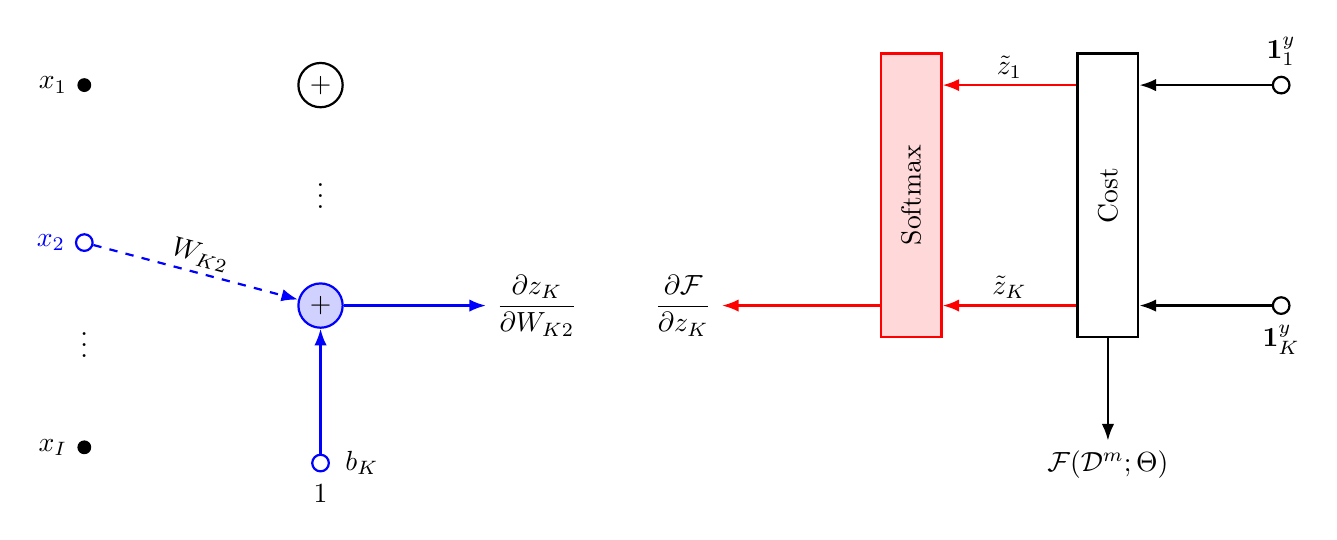
\begin{tikzpicture}[>=Latex]

    % ===== left cluster: forward-pass derivation for W_{K2}, b_K (blue) =====

    % inputs (x_2 highlighted)
    \node[unit, label=left:{$x_1$}] (x1) at (0, 3)  {};
    \node[circle, draw=fwdblue, thick, fill=white, minimum size=6pt, inner sep=0pt,
          label=left:{\textcolor{fwdblue}{$x_2$}}] (x2) at (0, 1) {};
    \node                            (xd) at (0, -0.2) {$\vdots$};
    \node[unit, label=left:{$x_I$}] (xI) at (0, -1.6) {};

    % sum nodes: top plain, bottom highlighted
    \node[sumop] (sA) at (3, 3) {$+$};
    \node        (sd) at (3, 1.7) {$\vdots$};
    \node[sumop, draw=fwdblue, fill=fwdblue!18] (sB) at (3, 0.2) {$+$};

    % highlighted weight edge and bias
    \draw[edge, fwdblue, dashed] (x2) -- (sB)
        node[wire, midway, above, sloped, black] {$W_{K2}$};
    \node[circle, draw=fwdblue, thick, fill=white, minimum size=6pt, inner sep=0pt]
        (bK) at (3, -1.8) {};
    \node[right=2pt of bK] {$b_K$};
    \node[below=1pt of bK] {$1$};
    \draw[edge, fwdblue] (bK) -- (sB);

    % forward output derivative
    \draw[edge, fwdblue] (sB) -- ++(2.1, 0)
        node[right, black] {$\dfrac{\partial z_K}{\partial W_{K2}}$};

    % ===== right cluster: backprop through softmax / cost (red) =====
    \node[opbox, minimum height=3.6cm, draw=bpred, fill=bpred!15]
        (soft) at (10.5, 1.6) {\vlabel{Softmax}};
    \node[opbox, minimum height=3.6cm] (cost) at (13.0, 1.6) {\vlabel{Cost}};

    \coordinate (yT) at (0, 3.0);
    \coordinate (yB) at (0, 0.2);

    % backprop cost -> softmax (red, leftward)
    \draw[edge, bpred] (cost.west |- yT) -- (soft.east |- yT)
        node[wire, midway, above, black] {$\tilde{z}_1$};
    \draw[edge, bpred] (cost.west |- yB) -- (soft.east |- yB)
        node[wire, midway, above, black] {$\tilde{z}_K$};

    % indicator inputs (black, leftward into cost)
    \node[circle, draw, thick, fill=white, minimum size=6pt, inner sep=0pt,
          label=above:{$\mathbf{1}^y_1$}] (i1) at (15.2, 3.0) {};
    \node[circle, draw, thick, fill=white, minimum size=6pt, inner sep=0pt,
          label=below:{$\mathbf{1}^y_K$}] (iK) at (15.2, 0.2) {};
    \draw[edge] (i1) -- (cost.east |- i1);
    \draw[edge] (iK) -- (cost.east |- iK);

    % backprop output of softmax (red, leftward)
    \draw[edge, bpred] (soft.west |- yB) -- ++(-2.0, 0)
        node[left, black] {$\dfrac{\partial \mathcal{F}}{\partial z_K}$};

    % cost forward output (black, down)
    \draw[edge] (cost.south) -- ++(0, -1.3)
        node[below] {$\mathcal{F}(\mathcal{D}^m; \Theta)$};

\end{tikzpicture}
\end{document}
